\chapter{VGMLの実装}\label{cha:Implementation}

本研究では、\ref{cha:Function}節で示した、既存手法の課題を解決するために、VDM++仕様書における以下の4つの構文を生成する手法を提案する。
さらに、提案手法を既存手法に適用し、機械学習を活用したVDM++仕様書自動生成ツールVGMLを開発する。

\begin{itemize}
    \item クラス
    \item インスタンス変数定義
    \item 関数定義
    \item 操作定義
\end{itemize}

本研究で開発するVGMLの構造を、図\ref{}に示す。以降、4つの構文の生成手法について詳細を説明する。

\section{クラスへの対応}
本節では、自然言語仕様書からVDM++仕様書におけるクラスを生成する手法を提案する。具体的には、既存手法の処理部である変換部と機械学習部に対して以下の改良を行う。

\begin{itemize}
    \item 変換部の自然言語仕様書内の単語にパラメータを追加する処理の改良。
    \item 機械学習部の学習済みモデルを生成する処理を改良。
    \item 機械学習部の自然言語仕様書内の単語を分類する処理を改良。
\end{itemize}

以降、3つの改良について詳細を述べる。

\subsection{自然言語仕様書内の単語にパラメータを追加する処理の改良}
既存手法は、図\ref{}に示す変換部において、各単語にTF-IDF値、出現回数、優先値、連結回数の4つの値を追加する。
さらに、図\ref{}に示す単語リストを生成する。
既存手法が生成する単語リストは、単語名と、各単語に対して算出した、TF-IDF値、出現回数、優先値、連結回数の4つのパラメータを持つ。
これにより、機械学習によって自然言語内の単語を、VDM++仕様書に必要である単語と、必要でない単語に分類することができる。

VGMLの変換部の構造を図\ref{}に、VGMLが生成する単語リストを図\ref{}にそれぞれ示す。
VGMLは、図\ref{}に示す概念レベル算出処理において、本論文で新たに定義する概念レベルを計算する。
さらに、変換部の概念レベル生成処理において、各単語に新たなパラメータとして概念レベルを追加し、図\ref{}に示す単語リストを生成する。
VGMLが生成する単語リストは、単語名と、各単語に対して算出した、TF-IDF値、出現回数、優先値、連結回数、概念レベルの5つのパラメータを持つ。
これにより、機械学習によって自然言語仕様書内の単語を、VDM++仕様書に必要でない単語、VDM++仕様書に必要であるが、クラスの候補ではない単語、
VDM++仕様書に必要であり、かつ、クラスの候補である単語の3つに分類することができる。
以降、概念レベル算出処理と概念レベル生成処理の詳細について説明する。

概念レベルの計算は、\ref{}で述べた日本語WordNetを用いて、解析対象である単語とその下位概念の関係を表す木構造を生成する。
単語の下位概念の関係を表す木構造の例を、図\ref{}に示す。図\ref{}は、"りんご"の文字列を入力した際の木構造の例である。
日本語WordNetは、日本語での入力に対応しているが、出力する概念を表す単語は英語表記であるため、木構造を構成する単語も英語表記となる。
図\ref{}の木構造の場合、りんごの概念を持つ単語を最上位のノードとし、その下位概念である単語を子ノードとして表現する。

概念レベル算出部における概念レベル算出処理の流れを、以下に示す。
\begin{enumerate}
    \item 単語を入力として読み込む。
    \item 
\end{enumerate}


\begin{figure}[t]
    \begin{center}
        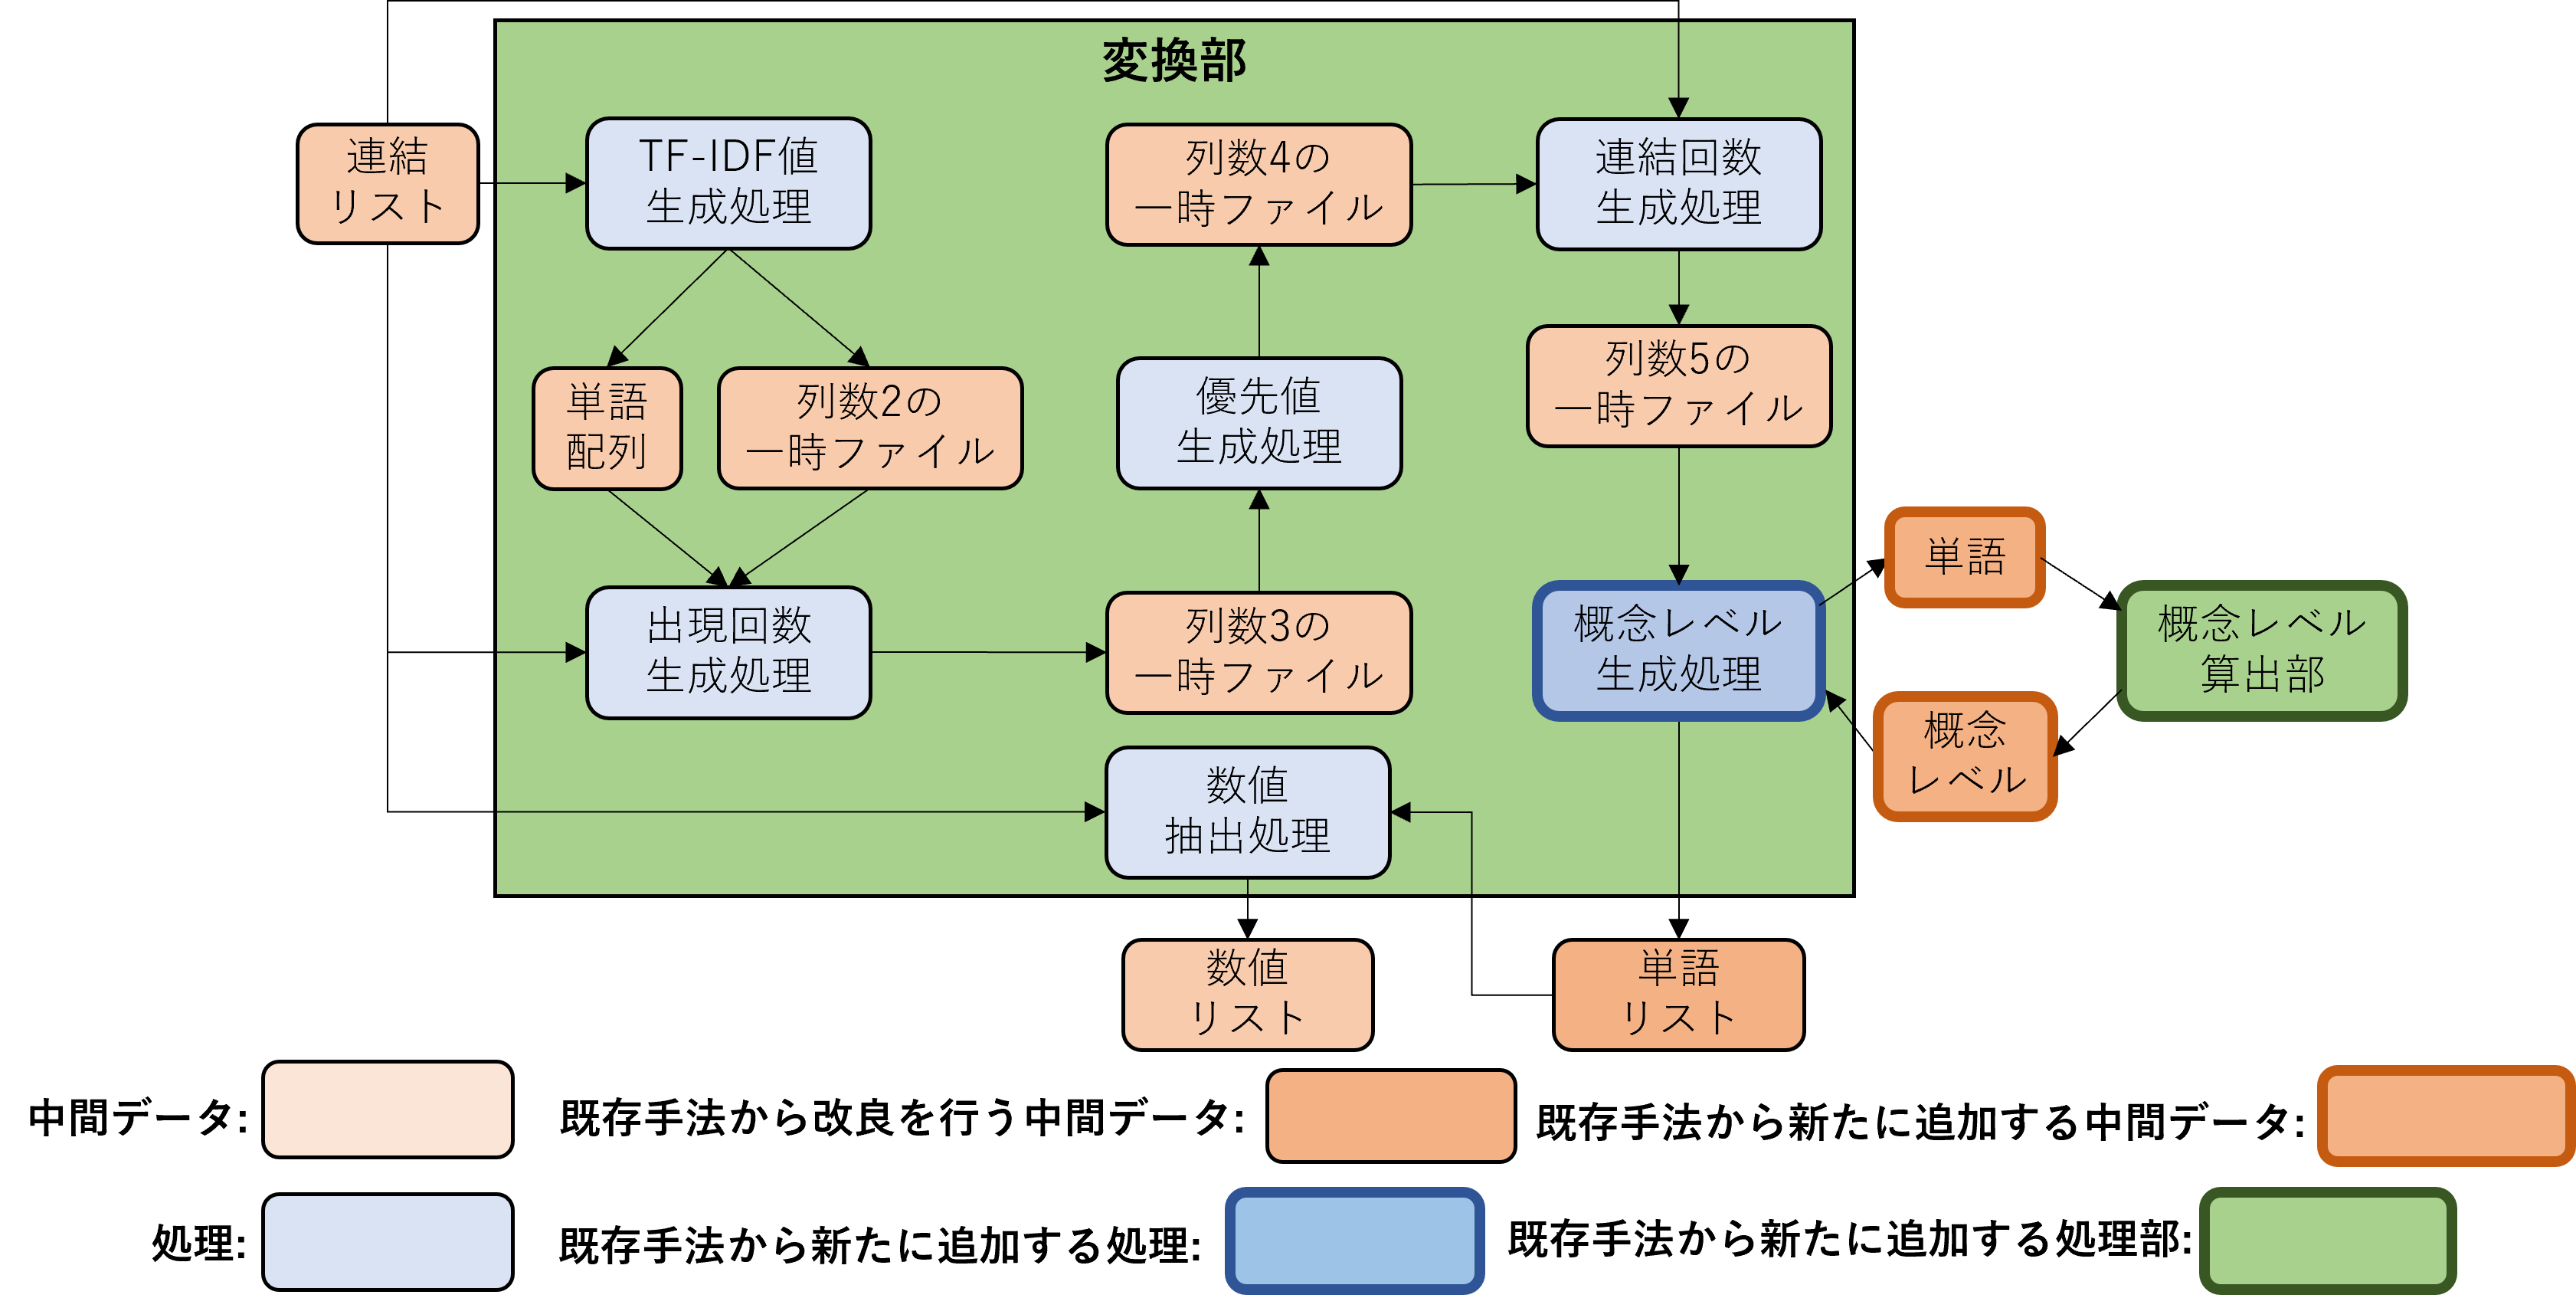
\includegraphics[width=1.0\columnwidth]{image/vgml_transfer.png}
        \caption{VGMLの変換部の構造}
        \label{fig:sample}
    \end{center}
\end{figure}

VGMLにおける変換部の概念レベル生成処理の流れを、以下に示す。

\begin{itemize}
    \item 
\end{itemize}